\documentclass{beamer}
\usepackage{array}
\usepackage{graphicx}
\usepackage{xcolor}
\usepackage{graphicx}
\usepackage{amsmath}

\usetheme{Madrid}

% Suppress the navigation bar and remove name and date from slides
\setbeamertemplate{navigation symbols}{}
\setbeamertemplate{footline}{}  % Removes the footer line with the author and date
\setbeamertemplate{headline}{}  % Removes the header line

% Title page details
\title{Conversational Used Car Price Predictor}
\subtitle{CS702 - Computing Lab}
\author{ABHIJITH C \and ANAND M K}
\institute{Department of Computer Science and Engineering \\ NITK Surathkal}
\date{}  % No date on title slide

\begin{document}

% Title page
\begin{frame}[t]
    \titlepage
\end{frame}

\begin{frame}[t]{Introduction}
    \begin{itemize}
        \item This project focuses on developing a \textbf{Conversational Used Car Price Predictor}, integrating a chatbot interface with a machine learning model.
        \item \textbf{Goal:} To allow users to interact through natural conversation rather than filling out traditional forms to predict used car prices.
        \item The chatbot will collect necessary car details (brand, model, year, mileage, etc.) step by step through an intuitive and engaging interface.
        \item A machine learning model will use the gathered data to predict the price of the used car, ensuring accurate and reliable predictions.
        \item The chatbot also handles additional queries, such as explaining how the price was calculated or what factors affect the car’s value.
    \end{itemize}
\end{frame}


\begin{frame}{System Architecture}'
    \centering
   	 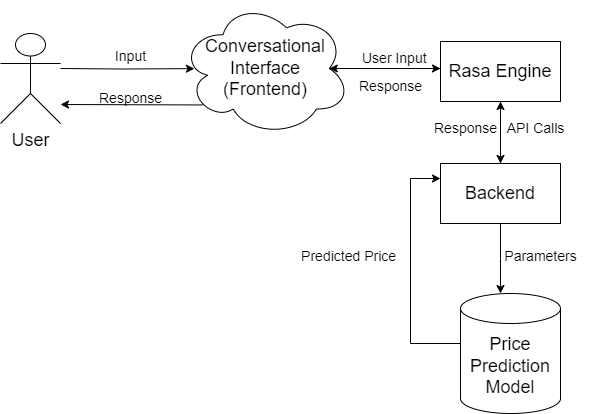
\includegraphics[width=0.8\textwidth]{Midsem.drawio.png}
\end{frame}

\begin{frame}{System Flow Explanation}
    \begin{itemize}
        \item The user interacts with the system via a chat interface in the frontend, initiating a conversation to predict the price of their used car.
        \item The user inputs (car details such as make, model, year, mileage, etc.) are processed by the \textbf{Rasa Engine}, which handles NLP and conversation management.
        \item The Rasa Engine extracts relevant parameters from the conversation and sends them to the backend, where the \textbf{Price Prediction Model} calculates the car's estimated price based on the input features.
        \item \textbf{SHAP} (SHapley Additive exPlanations) is applied to explain the contribution of each feature (e.g., mileage, car age, etc.) to the final price prediction, identifying the most impactful factor.
        \item The backend returns both the predicted price and the explanation of the most significant contributing factor, which are displayed to the user through the chat interface.
    \end{itemize}
\end{frame}


\begin{frame}{Project Overview: Progress and Next Steps}
    \begin{itemize}
        \item \textbf{Milestones Achieved:}
        \begin{itemize}
            \item Data collection and preprocessing for the car price prediction model.
            \item Model development using \textbf{Random Forest} and SHAP calculation for feature contribution analysis.
            \item Backend API to return the predicted price and the maximum contributing feature.
            \item Development of a sample chatbot to collect car parameters from the user.
        \end{itemize}
        
        \item \textbf{\textcolor{gray}{Upcoming Work:}}
        \begin{itemize}
            \item \textcolor{gray}{Improve the Rasa chatbot by adding more test data.}
            \item \textcolor{gray}{Validation of user input parameters in the Rasa chatbot.}
            \item \textcolor{gray}{Handle general questions in Rasa.}
            \item \textcolor{gray}{Integration of the backend with Rasa.}
            \item \textcolor{gray}{Frontend integration with Rasa for seamless user interaction.}
        \end{itemize}
    \end{itemize}
\end{frame}

\begin{frame}{Data Preprocessing Steps (Part 1)}
    \begin{itemize}
        \item \textbf{Finding the Dataset:} 
        \begin{itemize}
            \item Dataset sourced from Kaggle: \texttt{cardekho\_dataset} in 2023.
        \end{itemize}
        
        \item \textbf{Dropping Unnecessary Columns:}
        \begin{itemize}
            \item Removed columns such as \texttt{"Unnamed: 0"} (irrelevant index) and \texttt{"car\_name"} (redundant feature).
        \end{itemize}
        
        \item \textbf{Converting Vehicle Age to Year of Manufacture:}
        \begin{itemize}
            \item Calculated \texttt{year\_of\_manufacture} using the formula: 
            \[ \texttt{year\_of\_manufacture} = 2023 - \texttt{vehicle\_age} \]
            \item Dropped the \texttt{vehicle\_age} column.
        \end{itemize}
        
        \item \textbf{Filtering Popular Car Models:}
        \begin{itemize}
            \item Filtered the dataset to retain models with more than 300 entries, ensuring sufficient data for model training.
        \end{itemize}
    \end{itemize}
\end{frame}

\begin{frame}{Data Preprocessing Steps (Part 2)}
    \begin{itemize}
        \item \textbf{Feature (X) and Target (y) Definition:}
        \begin{itemize}
            \item Defined \texttt{X} (features) by dropping \texttt{selling\_price} and \texttt{seller\_type}.
            \item Defined \texttt{y} as the \texttt{selling\_price} (target variable).
        \end{itemize}
        
        \item \textbf{Categorical Columns:}
        \begin{itemize}
            \item Identified categorical features like \texttt{fuel\_type}, \texttt{transmission\_type}, \texttt{brand}, and \texttt{model} that need encoding.
        \end{itemize}
        
        \item \textbf{Data Splitting:}
        \begin{itemize}
            \item Split the dataset into 80\% training and 20\% test sets using \texttt{train\_test\_split()}, ensuring reproducibility with \texttt{random\_state=42}.
        \end{itemize}
        
        \item \textbf{Preprocessing Pipeline (One-Hot Encoding):}
        \begin{itemize}
            \item Used \texttt{ColumnTransformer} to apply \texttt{OneHotEncoder} to categorical columns, converting them into binary variables for model compatibility.
        \end{itemize}
    \end{itemize}
\end{frame}

\begin{frame}{Model Training Process (Part 1)}
    \begin{itemize}
        \item \textbf{Model Selection:}
        \begin{itemize}
            \item A \textbf{Random Forest Regressor} was chosen for car price prediction.
            \item The model is robust, handles non-linear data well, and is less prone to overfitting.
        \end{itemize}
        
        \item \textbf{Pipeline Setup:}
        \begin{itemize}
            \item A pipeline was created to seamlessly combine preprocessing and model training.
            \item Ensures that the same transformations are applied during both training and testing.
        \end{itemize}
        
        \item \textbf{Hyperparameter Tuning:}
        \begin{itemize}
            \item \textbf{RandomizedSearchCV} was employed to efficiently search for the best hyperparameters.
            \item This method randomly samples a specified number of hyperparameter combinations from the defined parameter grid.
        \end{itemize}
    \end{itemize}
\end{frame}

\begin{frame}{Model Training Process (Part 2)}
    \begin{itemize}
        \item \textbf{Hyperparameter Tuning (continued):}
        \begin{itemize}
            \item Parameters tuned included:
            \begin{itemize}
                \item \texttt{n\_estimators}: Number of trees in the forest (100, 200, 300).
                \item \texttt{max\_depth}: Maximum tree depth (None, 10, 20, 30).
                \item \texttt{min\_samples\_split}: Minimum samples to split (2, 5, 10).
                \item \texttt{min\_samples\_leaf}: Minimum samples at each leaf (1, 2, 4).
            \end{itemize}
            \item \textbf{n\_iter=10}: Specifies the number of different combinations to try.
        \end{itemize}

        \item \textbf{Cross-validation:}
        \begin{itemize}
            \item \textbf{5-fold cross-validation} was used to evaluate model performance.
            \item This process repeats 5 times, with each fold serving as the test set once.
            \item Final performance is averaged over the 5 iterations for robust evaluation.
        \end{itemize}
        
        \item \textbf{Results:}
        \begin{itemize}
            \item The best model was selected based on the \textbf{R² Score: 0.925} on the test set.
            \item The best model was saved for future predictions.
        \end{itemize}
    \end{itemize}
\end{frame}

\begin{frame}{SHAP Value Calculation}
    \begin{itemize}
        \item \textbf{SHAP Value Calculation:}
        \begin{itemize}
            \item SHAP (SHapley Additive exPlanations) is a method used to explain the output of machine learning models by assigning each feature a contribution value for a particular prediction.
            \item An \texttt{Explainer} object is created for the trained Random Forest model using SHAP.
            \item SHAP values are computed for the transformed input data, representing how much each feature pushed the prediction higher or lower than the average model output.
        \end{itemize}
        \vspace{5pt}
        
        \item \textbf{Analyzing SHAP Values:}
        \begin{itemize}
            \item SHAP values are organized into a DataFrame, providing a clear breakdown of each feature’s contribution to the predicted price.
            \item Positive SHAP values indicate features that push the predicted price higher, while negative values indicate features that pull the price lower.
        \end{itemize}
    \end{itemize}
\end{frame}

\begin{frame}{Identifying Influential Features}
    \begin{itemize}
        \item \textbf{Identifying the Most Influential Feature:}
        \begin{itemize}
            \item The feature with the highest SHAP value is identified as the most influential factor in determining the predicted price for that specific car.
            \item This feature typically has the largest impact on driving the predicted price up or down.
        \end{itemize}
        \vspace{5pt}
        
        \item \textbf{Percentage Contribution Calculation:}
        \begin{itemize}
            \item The SHAP value of the most influential feature is divided by the predicted price to calculate its percentage contribution.
            \item This provides a more intuitive understanding of how much influence the top feature has on the final predicted price.
        \end{itemize}
        \vspace{5pt}
        
        \item \textbf{Feature Attribution:}
        \begin{itemize}
            \item The system outputs both the predicted price and the feature with the highest contribution, along with the percentage of its influence.
            \item This gives users a clear explanation of why the price is what it is, based on the input features.
        \end{itemize}
    \end{itemize}
\end{frame}


\begin{frame}{Backend API Creation}
    \begin{itemize}
        \item \textbf{Framework Used:} Flask
        \begin{itemize}
            \item A lightweight web framework for Python, used to create web applications.
        \end{itemize}
        
        \item \textbf{Endpoints:}
        \begin{itemize}
            \item \texttt{/predict\_price}: 
            \begin{itemize}
                \item Accepts car attributes as query parameters.
                \item Returns the predicted selling price of the car.
            \end{itemize}
            \item \texttt{/max\_contribution}: 
            \begin{itemize}
                \item Accepts the same car attributes as query parameters.
                \item Returns the highest contributing feature to the predicted price and its percentage contribution.
            \end{itemize}
        \end{itemize}
        
        \item \textbf{Input Handling:}
        \begin{itemize}
            \item Retrieves input data via query parameters (GET API).
        \end{itemize}
        
        \item \textbf{Response Format:}
        \begin{itemize}
            \item Outputs predictions and contributions as JSON, facilitating easy integration with frontend applications.
        \end{itemize}
    \end{itemize}
\end{frame}

\begin{frame}
\frametitle{Chatbot Development}
\begin{itemize}
 	\item The chatbot utilizes Rasa, an open-source machine learning framework, which enables the creation of conversational agents. The following configuration files are used to define intents, entities, slots, responses, and actions for the chatbot.
\end{itemize}
\end{frame}

\begin{frame}
\frametitle{Domain Configuration}
The \texttt{domain.yml} file defines the chatbot's intents, entities, and responses.

\begin{itemize}
    \item \textbf{Intents:} These are the goals of the user's input, such as greetings, farewells, and car information.
    \item \textbf{Entities:} Specific pieces of information extracted from the user's input, such as the brand and model of the car.
    \item \textbf{Slots:} Temporary storage for extracted entities, enabling the bot to remember information throughout the conversation.
    \item \textbf{Responses:} Predefined replies the bot can use to interact with users.
\end{itemize}
\end{frame}

\begin{frame}
\frametitle{Natural Language Understanding (NLU)}
The \texttt{nlu.yml} file contains examples of user intents and how to recognize entities within those intents. It includes:

\begin{itemize}
    \item \textbf{Intent Examples:} For greetings, farewells, and inquiries about the bot's identity.
    \item \textbf{Informing Brand and Model:} Recognizing car brand and model through user input, enabling the bot to process vehicle information accurately.
\end{itemize}
\end{frame}

\begin{frame}
\frametitle{Rules and Stories}
The \texttt{rules.yml} file defines specific rules for the conversation flow, while the \texttt{stories.yml} file illustrates the conversation paths. Together, they guide the bot's responses based on user interactions.

\begin{itemize}
    \item \textbf{Rules:} Trigger actions based on specific intents, such as saying goodbye or responding to bot challenges.
    \item \textbf{Stories:} Represent various user interaction scenarios, illustrating how the bot should respond.
\end{itemize}
\end{frame}

\begin{frame}
\frametitle{Custom Actions}
The \texttt{actions.py} file contains custom actions that allow the bot to perform specific tasks, such as storing user information.
\begin{itemize}
    \item \textbf{ActionStoreBrand:} Captures the brand of the car from user input and stores it in a slot.
    \item \textbf{ActionStoreModel:} Similar functionality for capturing the car model.
\end{itemize}
\end{frame}

\begin{frame}{Upcoming Work}
    \begin{itemize}
        \item Improve the Rasa chatbot by adding more test data to enhance its understanding and responsiveness.
        \item Validate user input parameters to ensure accurate and reliable data collection for predictions.
        \item Handle general questions within the chatbot to improve user engagement and satisfaction.
        \item Integrate the backend with Rasa for real-time access to the price prediction model.
        \item Implement frontend integration with Rasa for a seamless user interaction experience.
    \end{itemize}
\end{frame}


\begin{frame}[t]{References}
\begin{thebibliography}{9}

\bibitem{rasa}
Rasa Technologies, ``Rasa Documentation,'' \textit{Rasa}, 2023. [Online]. Available: \texttt{https://rasa.com/docs/}
\bibitem{flask}
Armin Ronacher, ``Flask Documentation,'' \textit{Flask}, 2023. [Online]. Available: \texttt{https://flask.palletsprojects.com/}


\bibitem{shap-doc}
SHAP Documentation, ``SHAP (SHapley Additive exPlanations),'' 2023. [Online]. Available: \texttt{https://shap.readthedocs.io/en/latest/}

\bibitem{randomforest}
Leo Breiman, ``Random Forests,'' \textit{Machine Learning}, vol. 45, no. 1, 2001, pp. 5-32. [Online]. Available: \texttt{https://link.springer.com/article/10.1023/A:1010933404324}

\bibitem{randomforest-doc}
Scikit-learn, ``Random Forests,'' 2023. [Online]. Available: \texttt{https://scikit-learn.org/dev/modules/generated/\\sklearn.ensemble.RandomForestRegressor.html}



\end{thebibliography}
\end{frame}



\begin{frame}[t]{.}
    \centering
    \vspace{1cm}
    \textbf{\Huge{}}
    
    \vspace{0.5cm}
    \rule{0.5\textwidth}{0.5mm} % Horizontal line for design

    \vspace{1cm}
    \textbf{\Large{Thank You!}}

    \vspace{0.5cm}
    \rule{0.5\textwidth}{0.5mm} % Another horizontal line for symmetry
\end{frame}


\end{document}
